\tikzset{every picture/.style={line width=0.75pt}} %set default line width to 0.75pt        

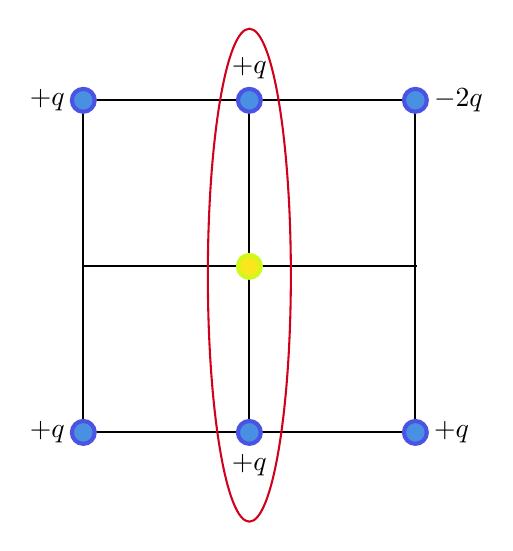
\begin{tikzpicture}[x=0.75pt,y=0.75pt,yscale=-1,xscale=1]
%uncomment if require: \path (0,430); %set diagram left start at 0, and has height of 430

%Shape: Grid [id:dp9511403020531122] 
\draw  [draw opacity=0] (225,103) -- (386,103) -- (386,264) -- (225,264) -- cycle ; \draw   (225,103) -- (225,264)(305,103) -- (305,264)(385,103) -- (385,264) ; \draw   (225,103) -- (386,103)(225,183) -- (386,183)(225,263) -- (386,263) ; \draw    ;
%Shape: Circle [id:dp026055485587581195] 
\draw  [color={rgb, 255:red, 74; green, 83; blue, 226 }  ,draw opacity=1 ][fill={rgb, 255:red, 74; green, 144; blue, 226 }  ,fill opacity=1 ][line width=1.5]  (219.5,103) .. controls (219.5,99.96) and (221.96,97.5) .. (225,97.5) .. controls (228.04,97.5) and (230.5,99.96) .. (230.5,103) .. controls (230.5,106.04) and (228.04,108.5) .. (225,108.5) .. controls (221.96,108.5) and (219.5,106.04) .. (219.5,103) -- cycle ;
%Shape: Circle [id:dp8849353673163125] 
\draw  [color={rgb, 255:red, 74; green, 83; blue, 226 }  ,draw opacity=1 ][fill={rgb, 255:red, 74; green, 144; blue, 226 }  ,fill opacity=1 ][line width=1.5]  (299.5,103) .. controls (299.5,99.96) and (301.96,97.5) .. (305,97.5) .. controls (308.04,97.5) and (310.5,99.96) .. (310.5,103) .. controls (310.5,106.04) and (308.04,108.5) .. (305,108.5) .. controls (301.96,108.5) and (299.5,106.04) .. (299.5,103) -- cycle ;
%Shape: Circle [id:dp7298663131993588] 
\draw  [color={rgb, 255:red, 74; green, 83; blue, 226 }  ,draw opacity=1 ][fill={rgb, 255:red, 74; green, 144; blue, 226 }  ,fill opacity=1 ][line width=1.5]  (379.5,103) .. controls (379.5,99.96) and (381.96,97.5) .. (385,97.5) .. controls (388.04,97.5) and (390.5,99.96) .. (390.5,103) .. controls (390.5,106.04) and (388.04,108.5) .. (385,108.5) .. controls (381.96,108.5) and (379.5,106.04) .. (379.5,103) -- cycle ;
%Shape: Circle [id:dp5118102160520555] 
\draw  [color={rgb, 255:red, 74; green, 83; blue, 226 }  ,draw opacity=1 ][fill={rgb, 255:red, 74; green, 144; blue, 226 }  ,fill opacity=1 ][line width=1.5]  (219.5,263) .. controls (219.5,259.96) and (221.96,257.5) .. (225,257.5) .. controls (228.04,257.5) and (230.5,259.96) .. (230.5,263) .. controls (230.5,266.04) and (228.04,268.5) .. (225,268.5) .. controls (221.96,268.5) and (219.5,266.04) .. (219.5,263) -- cycle ;
%Shape: Circle [id:dp9003932477737502] 
\draw  [color={rgb, 255:red, 74; green, 83; blue, 226 }  ,draw opacity=1 ][fill={rgb, 255:red, 74; green, 144; blue, 226 }  ,fill opacity=1 ][line width=1.5]  (299.5,263) .. controls (299.5,259.96) and (301.96,257.5) .. (305,257.5) .. controls (308.04,257.5) and (310.5,259.96) .. (310.5,263) .. controls (310.5,266.04) and (308.04,268.5) .. (305,268.5) .. controls (301.96,268.5) and (299.5,266.04) .. (299.5,263) -- cycle ;
%Shape: Circle [id:dp7160989607764205] 
\draw  [color={rgb, 255:red, 74; green, 83; blue, 226 }  ,draw opacity=1 ][fill={rgb, 255:red, 74; green, 144; blue, 226 }  ,fill opacity=1 ][line width=1.5]  (379.5,263) .. controls (379.5,259.96) and (381.96,257.5) .. (385,257.5) .. controls (388.04,257.5) and (390.5,259.96) .. (390.5,263) .. controls (390.5,266.04) and (388.04,268.5) .. (385,268.5) .. controls (381.96,268.5) and (379.5,266.04) .. (379.5,263) -- cycle ;
%Shape: Circle [id:dp693930431751913] 
\draw  [color={rgb, 255:red, 207; green, 248; blue, 28 }  ,draw opacity=1 ][fill={rgb, 255:red, 248; green, 231; blue, 28 }  ,fill opacity=1 ][line width=1.5]  (299.5,183) .. controls (299.5,179.96) and (301.96,177.5) .. (305,177.5) .. controls (308.04,177.5) and (310.5,179.96) .. (310.5,183) .. controls (310.5,186.04) and (308.04,188.5) .. (305,188.5) .. controls (301.96,188.5) and (299.5,186.04) .. (299.5,183) -- cycle ;
%Shape: Ellipse [id:dp5545063148136824] 
\draw  [color={rgb, 255:red, 208; green, 2; blue, 27 }  ,draw opacity=1 ] (305,68.5) .. controls (316.05,68.5) and (325,121.67) .. (325,187.25) .. controls (325,252.83) and (316.05,306) .. (305,306) .. controls (293.95,306) and (285,252.83) .. (285,187.25) .. controls (285,121.67) and (293.95,68.5) .. (305,68.5) -- cycle ;

% Text Node
\draw (217.5,103) node [anchor=east] [inner sep=0.75pt]    {$+q$};
% Text Node
\draw (217.5,263) node [anchor=east] [inner sep=0.75pt]    {$+q$};
% Text Node
\draw (305,94.1) node [anchor=south] [inner sep=0.75pt]    {$+q$};
% Text Node
\draw (305,271.9) node [anchor=north] [inner sep=0.75pt]    {$+q$};
% Text Node
\draw (392.5,263) node [anchor=west] [inner sep=0.75pt]    {$+q$};
% Text Node
\draw (392.5,103) node [anchor=west] [inner sep=0.75pt]    {$-2q$};


\end{tikzpicture}
